\section{Results on the ordinary day}
\label{sec:results}

The ordinary day is a simulated day with no disruption, the day the survey describes. 
On that day the benchmark yields four findings, one per subsection.

\begin{enumerate}
  \item The decision-makers form groups, and a prompt with no general criteria
    already beats every baseline.
  \item The expert prompt improves every language model, aligning some dimensions of the
    modal split and leaving others untouched.
  \item A classifier that reads the same trip description and writes no text scores within
    the range of the four reference models.
  \item Agreement on the modal split does not carry over to individual trips.
\end{enumerate}

\subsection{Fifteen decision-makers form groups}
\label{sec:scale}

The fifteen decision-makers form distinct groups on the composite (Figure~\ref{fig:scale},
Table~\ref{tab:scale}). The uniform baseline has about fourteen times the error of the best
reference model. Every minimal-prompt condition already has less error than the three
baselines. The weakest minimal-prompt condition scores 14.8, compared with 27.0 for the best
baseline (minimum duration). A model that receives the facts of a trip, and no general
criteria, therefore holds behavioural information that the minimum-duration baseline lacks.
The four reference models hold the lowest errors. The typed classifier under its expert
prompt sits among them, at 3.65.

\begin{table*}[tp]
  \caption{The fifteen decision-makers on the two metrics, with the inter-seed range where it was measured. Rows are grouped, then sorted by composite.}
  \label{tab:scale}
  \begin{tabular}{llrrl}
    \toprule
    Group & Decision-maker & Composite & L1 on overall shares & Inter-seed range \\
    \midrule
    Baseline       & Uniform random                         & 50.16 & 86.80 & deterministic \\
    Baseline       & All-car                                & 30.73 & 58.00 & deterministic \\
    Baseline       & Minimum duration                       & 26.97 & 53.62 & deterministic \\
    Minimal prompt & \texttt{mistral-large}                 & 14.75 & 44.71 & [pending] \\
    Minimal prompt & typed classifier                       & 13.75 & 42.76 & 0.41 \\
    Minimal prompt & \texttt{gemini-3.1}                    & 12.38 & 39.88 & [pending] \\
    Minimal prompt & \texttt{gemini-3.5}                    &  7.02 & 24.08 & \textbf{[pending]} \\
    Expert prompt  & \texttt{gemini-3.1}                    &  8.98 & 31.25 & [pending] \\
    Expert prompt  & \texttt{mistral-large}                 &  7.63 & 26.64 & [pending] \\
    Expert prompt  & \texttt{gemini-3.5} (tuned agent)      &  4.86 & 13.85 & 0.56 \\
    Expert prompt  & typed classifier                       &  3.65 & 10.48 & 0.05 \\
    Reference      & Random forest                          &  4.09 &  5.28 & deterministic \\
    Reference      & Multinomial logit                      &  4.02 &  8.99 & deterministic \\
    Reference      & Kernel logistic regression             &  3.61 &  6.69 & deterministic \\
    Reference      & Gradient boosting                      &  3.60 &  9.49 & deterministic \\
    \bottomrule
  \end{tabular}
\end{table*}

The groups overlap in one place only: the best minimal-prompt condition, \texttt{gemini-3.5},
scores better than two expert-prompt conditions. It leads \texttt{gemini-3.1} under the
expert prompt by 2.0 composite points, and \texttt{mistral-large} under that prompt by 0.6, a
gap smaller than the cohort resolution.

The same prompt does not score the same on two versions of the same model family. With the
tuned agent's expert prompt left unchanged, \texttt{gemini-3.1} trails \texttt{gemini-3.5} by
4.2 composite points (95\,\% interval 3.0 to 5.4).

Re-running a condition with three seeds moves its composite less than the narrowest interval
half-width of Section~\ref{sec:quantities}, 0.9 points. The tuned agent varies by 0.6 points
across seeds (Table~\ref{tab:scale}). Under the minimal
prompt, the typed classifier varies by 0.4 points across seeds
(0.41), and by less than a quarter of a point under both expert prompts (0.05 and 0.24). The
sign of the difference between these two expert conditions holds on all three seeds. This
inter-seed variation of 0.4 points is small next to the gain from tuning the classifier's
prompt, which lowers the composite by 10.1 points (from 13.75 to 3.65).

\begin{figure*}[tp]
  \centering
  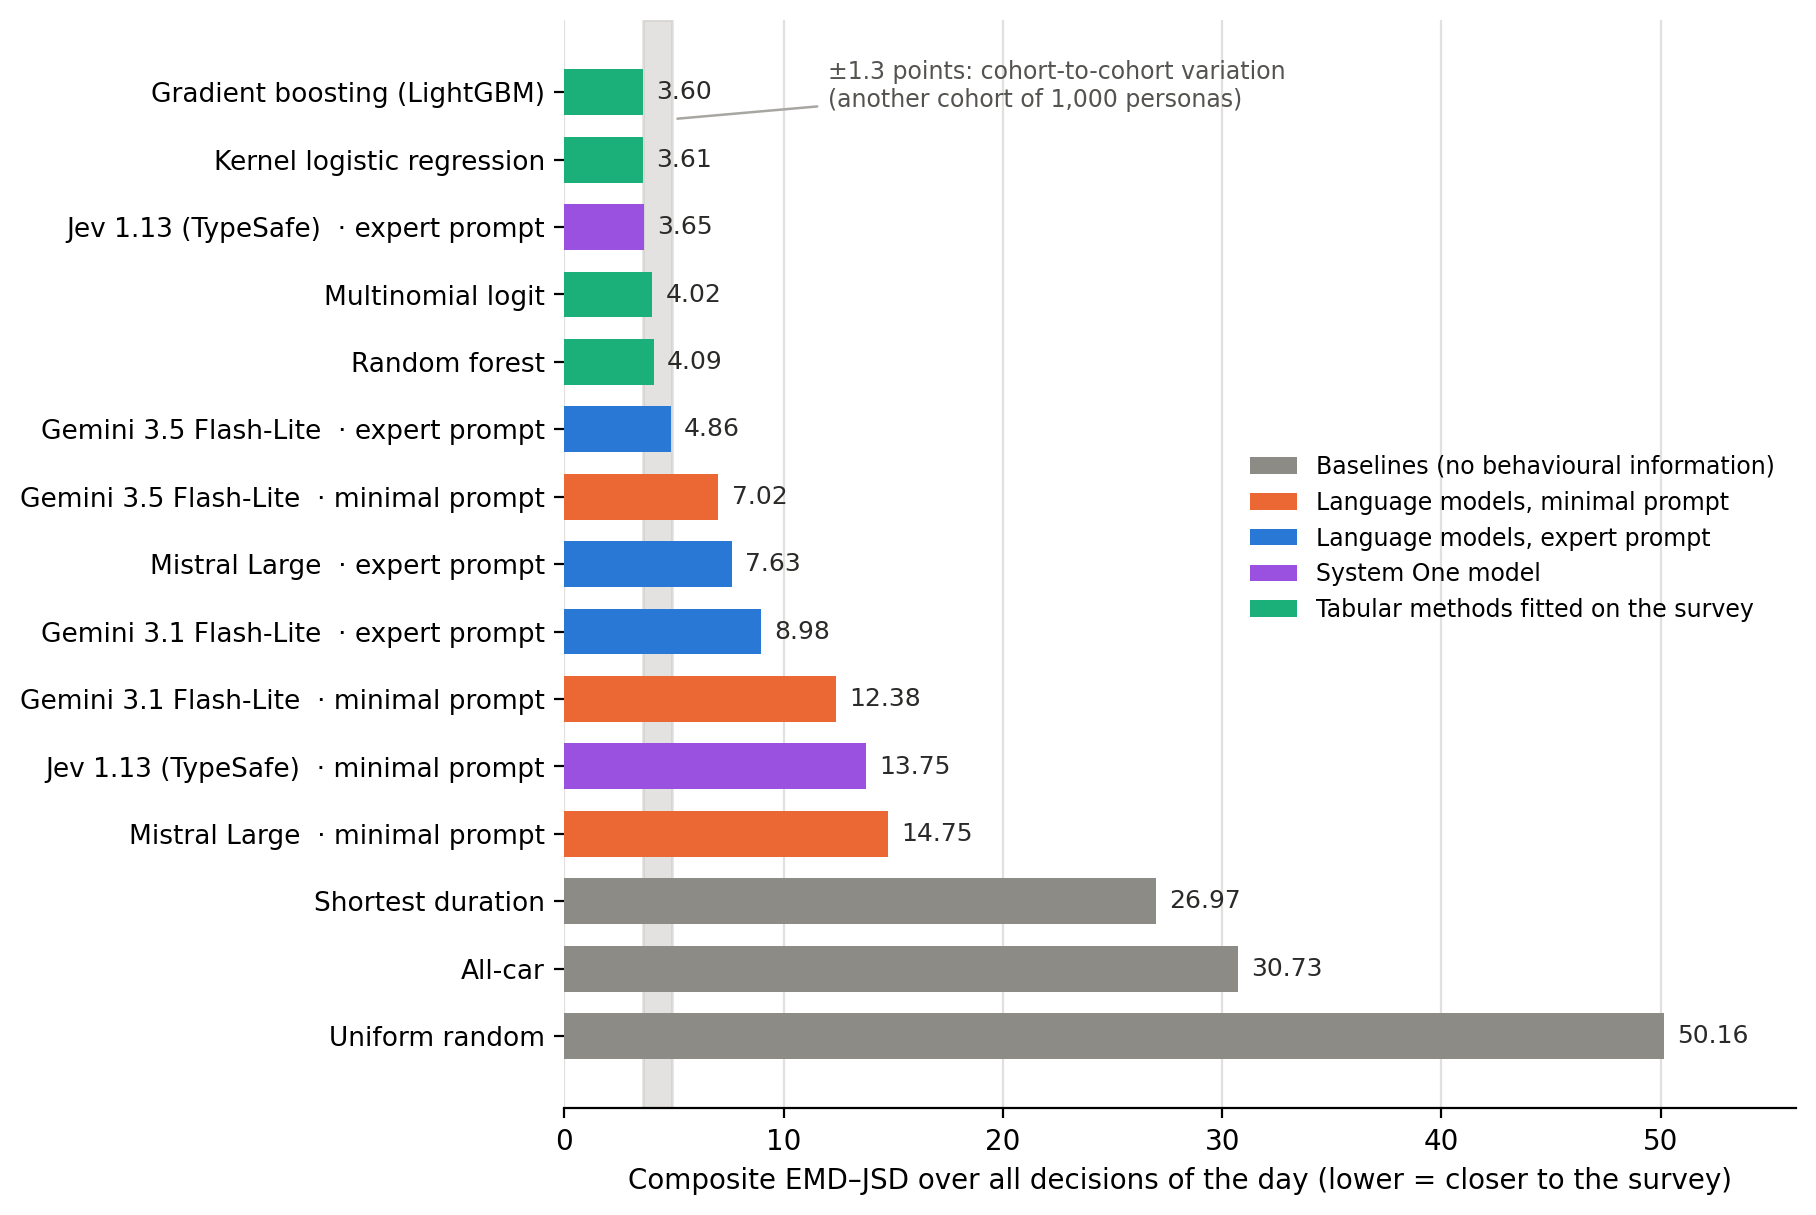
\includegraphics[width=\textwidth]{images/ch6_echelle.png}
  \caption{The decision-makers form groups on the composite axis, and even the minimal prompt has less error than the minimum-duration baseline. The grey band is the cohort resolution, the median half-width of a 95\,\% interval; it gives a scale, not a test.}
  \Description{A horizontal bar chart. The x axis is the composite EMD-JSD error over every decision of the day, running from zero on the left to just over fifty on the right; lower means closer to the survey. Fifteen decision-makers are stacked as rows and coloured by group, and each bar carries its value. Sorted from the best: gradient boosting 3.60, kernel logistic regression 3.61, the typed classifier under its expert prompt 3.65, the multinomial logit 4.02 and the random forest 4.09; then Gemini 3.5 Flash-Lite under the expert prompt at 4.86, Gemini 3.5 Flash-Lite under the minimal prompt at 7.02, Mistral Large under the expert prompt at 7.63, Gemini 3.1 Flash-Lite under the expert prompt at 8.98, Gemini 3.1 Flash-Lite under the minimal prompt at 12.38, the typed classifier under the minimal prompt at 13.75 and Mistral Large under the minimal prompt at 14.75; at the far right the three baselines, minimum duration at 26.97, all-car at 30.73 and the uniform random draw at 50.16. A vertical grey band of about 1.3 points marks cohort-to-cohort variation, the median half-width of a 95 per cent interval. Gemini 3.5 Flash-Lite under the minimal prompt sits to the left of Gemini 3.1 Flash-Lite under the expert prompt by more than that band.}
  \label{fig:scale}
\end{figure*}

\subsection{What tuning changes, and what it does not}
\label{sec:tuning}

Tuning the system prompt lowers the error of all three models (Table~\ref{tab:gains}).
The paired gain runs from 2.3 to 7.3 composite
points, and all six intervals (three models, two metrics) exclude zero.

\begin{table*}[tp]
  \caption{Paired gains of the expert prompt over the minimal prompt, two metrics, with their 95\,\% interval in brackets. A positive gain is a lower error. Gains are computed on the persons both conditions scored, so they can differ slightly from the gaps in Table~\ref{tab:scale}.}
  % Écart au tableau 1 vérifié le 2026-09-25 : composite 2,27 / 3,37 / 7,25 contre 2,16 / 3,40 /
  %   7,12 par soustraction ; L1 10,2 / 8,6 / 18,0 identiques. Effet de l'appariement.
  \label{tab:gains}
  \begin{tabular}{lcc}
    \toprule
    Language model & Composite & L1 on overall shares \\
    \midrule
    \texttt{gemini-3.5}    & 2.27 [1.40, 3.22] & 10.2 [8.0, 12.5]  \\
    \texttt{gemini-3.1}    & 3.37 [2.45, 4.25] &  8.6 [6.8, 10.6]  \\
    \texttt{mistral-large} & 7.25 [5.90, 8.67] & 18.0 [13.5, 22.4] \\
    \bottomrule
  \end{tabular}
\end{table*}

Take \texttt{gemini-3.5} as an example, the model the expert prompt was tuned on. For this
model, tuning does not shift the car share uniformly (Figure~\ref{fig:distance}). Under one
kilometre the car share stays near 10\,\% before and after tuning, where the survey records
18\,\%. Between one and fifty kilometres it rises by six to seven points in every band. On the
distance stratum, the tuned agent then has less error than any reference model. Its L1 error,
taken within each distance class and averaged by class size, is 14.2 points. The random
forest, best of the four, scores 16.8. No other stratum gives an agent that lead.

The language models make two errors, and tuning corrects only one. They overestimate public
transport, and the expert prompt pulls it down by four to eleven points. They also
overestimate cycling, at 6.8 to 8.1\,\% where the survey records 4.1\,\%, and the expert
prompt moves the bike share by less than one point. No decision-maker fits one stratum: the
15--19-year-olds. The survey records 47.4\,\% public transport for them, compared with
26.4\,\% for the random forest and 20.8\,\% for the tuned agent (Appendix F).

\begin{figure}[tbp]
  \centering
  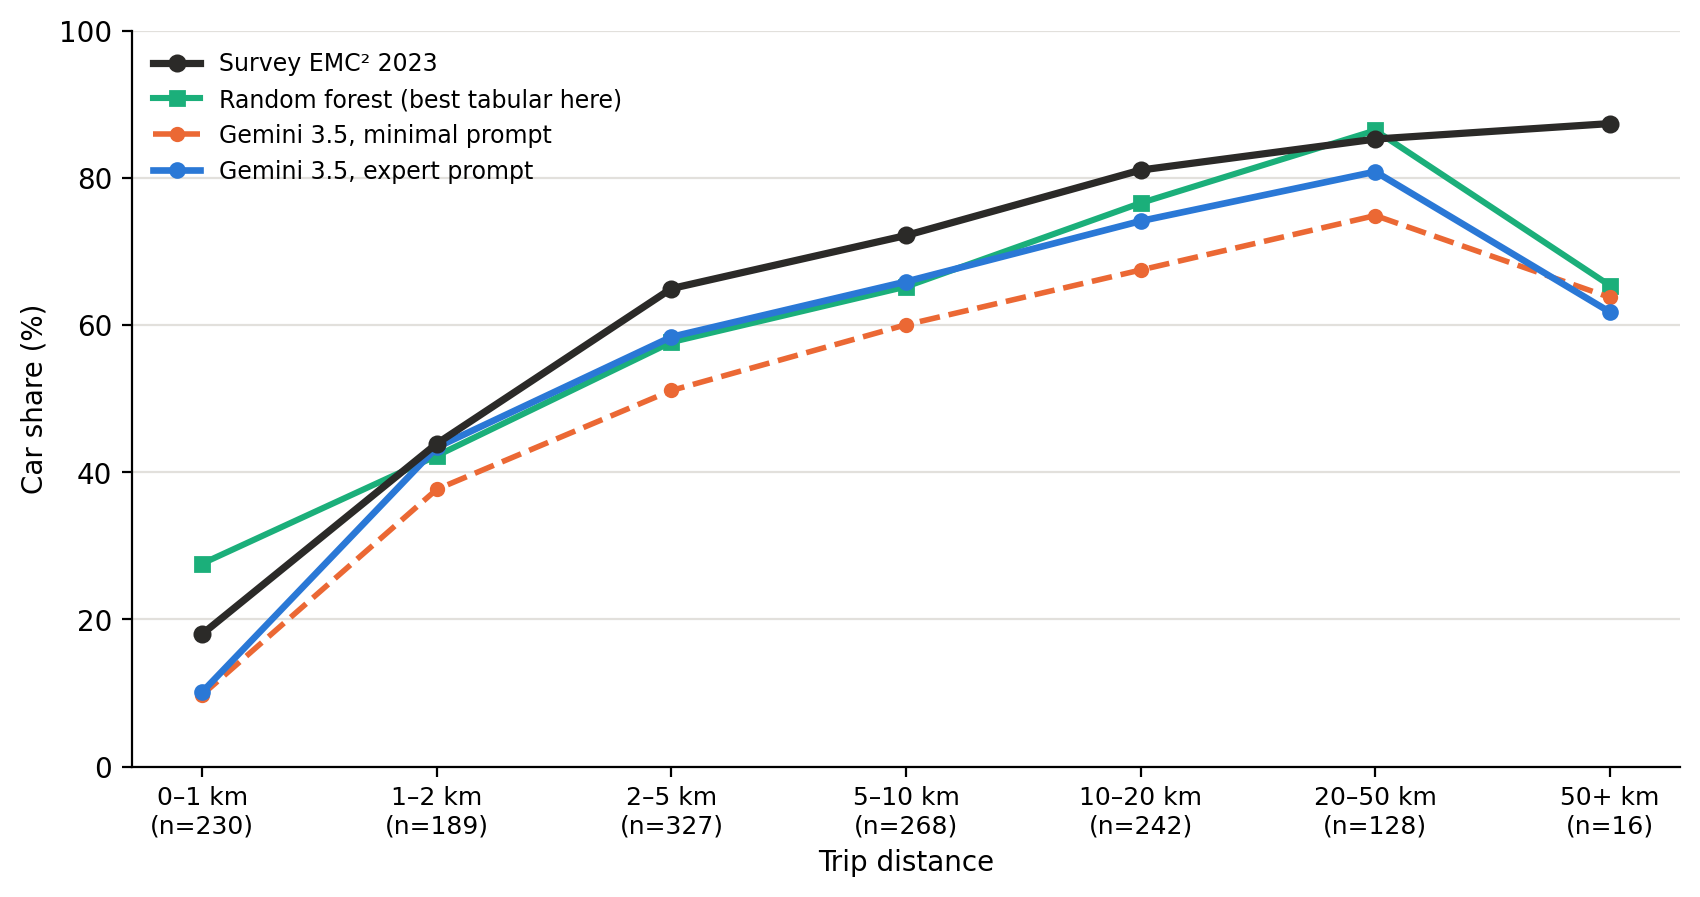
\includegraphics[width=\columnwidth]{images/ch6_distance.png}
  \caption{On \texttt{gemini-3.5}, tuning raises the car share beyond one kilometre, while the shortest trips stay where the minimal prompt left them.}
  \Description{A line chart with four series. The horizontal axis carries seven trip-distance bands, from zero to one kilometre up to more than fifty kilometres, each labelled with the number of trips it holds. The vertical axis is the car share in per cent, from zero to one hundred. The survey line climbs from 18 per cent on the shortest band to about 87 per cent on the longest. Gemini 3.5 Flash-Lite under the minimal prompt runs lowest throughout, from about 10 per cent to 75 per cent, then falls on the last band. The same model under the expert prompt starts at the same 10 per cent but rises faster, meeting the random forest from two kilometres on and staying five to ten points under the survey. The random forest alone starts high on the shortest band, at about 27 per cent, where the survey gives 18.}
  \label{fig:distance}
\end{figure}

\subsection{A classifier that writes no text reaches the reference range}
\label{sec:deliberation}

On the sealed cohort, the typed classifier under its expert prompt scores 3.65, inside the
range of the four reference models (3.60 to 4.09). On a second cohort of 1{,}000 personas,
drawn the same way with no persona in common, the four reference models span 2.53 to 3.71
composite points. The typed classifier scores 4.64 there, 0.9 points above that range.

The typed classifier thus reaches the reference range without writing text. Given the same
prompt as a language model, it is no longer clearly ahead. With the minimal prompt,
gemini-3.5 scores 7.02 and the classifier 13.75. With the tuned agent's prompt, the
classifier scores 4.14 and the agent 4.86, a gap smaller than a change of cohort. On the
second cohort, the two stand 0.1 points apart. This comparison therefore does not tell what
the text contributes.

For the same 23{,}026 decisions, the classifier costs \$1.06, whereas the tuned agent costs
\$49.28 at the standard rate, a factor of about fifty.

\subsection{Matching shares is not matching decisions}
\label{sec:individual}

The tuned agent and the gradient boosting model stand 1.3 composite points apart and still
disagree on one trip in three. They put their highest probability on a
different mode for 30.3\,\% of trips, counted where both saw at least two options. Between two
reference models the same count runs from 8.4 to 11.0\,\%. On the median trip, the summed
absolute gap between the mode probabilities of two generative agents is four times that of
two reference models.

On the reported days of the survey, the tuned agent predicts the reported mode slightly less
often than the reference models (Table~\ref{tab:unit}). It trails the gradient boosting model
by 3.9 accuracy points (95\,\% interval 2.3 to 5.5). No paired interval separates it from the
multinomial logit, on accuracy or on cross-entropy.

\begin{table}[tbp]
  \caption{Trip-level agreement on the reported days, seven decision-makers. Accuracy and recall in \%, on the 9{,}621 reported trips. Cross-entropy in nats, on the 5{,}229 decisions with at least two options that every distribution-valued decision-maker scores. The two baselines that return a single option receive none: a zero probability on the reported mode makes it infinite.}
  \label{tab:unit}
  \small
  \setlength{\tabcolsep}{4pt}
  \begin{tabularx}{\columnwidth}{@{}Lrrrr@{}}
    \toprule
    Decision-maker & \multicolumn{1}{c}{Acc.} & \multicolumn{1}{c}{Cross-} & \multicolumn{1}{c}{Bike} & \multicolumn{1}{c}{Walk} \\
                   &                          & \multicolumn{1}{c}{ent.}   & \multicolumn{1}{c}{rec.} & \multicolumn{1}{c}{rec.} \\
    \midrule
    Gradient boosting                                 & 71.5 & 0.299 & 20.4 & 63.4 \\
    Multinomial logit                                 & 68.6 & 0.358 & 18.3 & 60.0 \\
    Minimum duration                                  & 68.1 & ---   & 25.8 & 19.2 \\
    Expert prompt, \texttt{gemini-3.5}                & 67.6 & 0.341 & 22.5 & 47.2 \\
    All-car                                           & 66.7 & ---   &  2.3 & 16.2 \\
    Minimal prompt, \texttt{gemini-3.5}               & 64.8 & 0.384 & 24.1 & 44.2 \\
    Expert prompt, typed classifier                   & 64.7 & 0.464 & 18.1 & 56.3 \\
    \bottomrule
  \end{tabularx}
\end{table}

The typed classifier falls below the all-car baseline on individual accuracy. It trails that
baseline by 2.0 accuracy points (95\,\% interval 0.3 to 3.8), while its composite reaches the
range of the reference models (Section~\ref{sec:deliberation}). It over-predicts walking at
the expense of public transport. Its walk recall reaches 56.3\,\%, compared with about
44\,\% for public transport, and its walk precision falls below that of the two other
decision-makers (Figure~\ref{fig:audit-modes}). A population can therefore reproduce the
modal split of a territory while getting more individual trips wrong than a baseline that
takes the car whenever it can.

\begin{figure}[tbp]
  \centering
  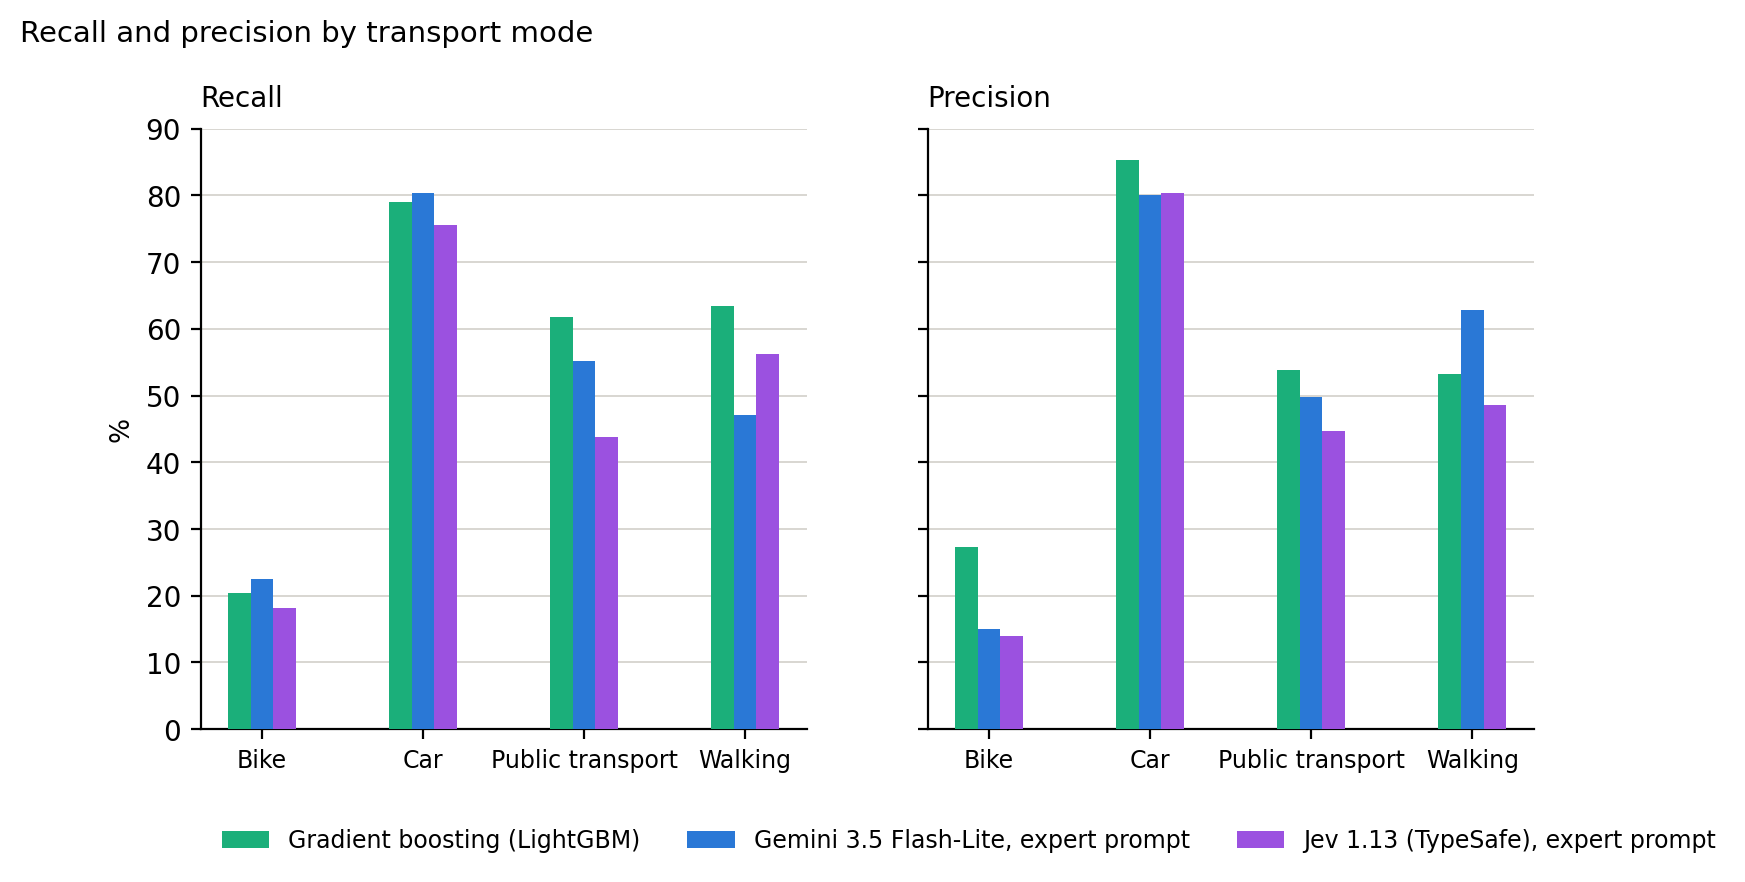
\includegraphics[width=\columnwidth]{images/ch6_audit_modes.png}
  \caption{Recall and precision by mode: the typed classifier trades public transport for walking, and the modal split does not show the exchange.}
  \Description{Two panels of grouped bars, recall on the left and precision on the right. In each panel the horizontal axis carries the four modes, bike, car, public transport and walking, and the vertical axis a percentage from zero to ninety. Three bars per mode: gradient boosting, the expert prompt on Gemini 3.5 Flash-Lite, and the typed classifier under the expert prompt. On the recall panel the typed classifier stands lowest on bike and on public transport, at about 18 and 44 per cent, and above the generative agent on walking, at about 56 per cent against 47. On the precision panel the relation reverses on walking, where the typed classifier falls under both others, and the three stay close on the car.}
  \label{fig:audit-modes}
\end{figure}

These four findings hold on the ordinary day the survey describes. A survey tabulates no
other day, and the next section moves beyond that day to an off-survey event.
